\section {The Z-Wave Device (JSON) API in detail}
\label{c2}

This chapter describes the Z-Wave Device API and its use in detail All examples 
will use the HTTP/JSON API notation. Please note that the C library notation offers 
equal functionality.

The Z-Wave Device API is the north-bound interface of the Z-Wave Core. This Z-Wave 
core implement the whole control logic of the Z-Wave network. The two main functions are

\begin{itemize}
\item Management of the network. This includes including and excluding devices, managing 
the routing and rerouting of the network an executing some housekeeping functions to 
keep the network clean and stable. The function classes can be seen as functions offered 
by the controller itself. Hence the variables and status parameters of the networks are 
offered by an object called ``controller.’’

\item Execution of commands offered by the wireless devices as such switching switches 
and dimming dimmers. Z-Wave groups the command and their corresponding variables into 
so-called command classes. The Z-Wave API offers access to these command classes with 
their variables and their commands according to the abilities of the respective device.
\end{itemize}

The description of function classes and command Cclasses and their access using the JSON 
API complete the description of the Z-Wave Device API. For a full reference of function 
classes and command classes please refer to the Annex \ref{FunctionClasses} and \ref{CommandClasses}.

\subsection{The data model}
\label{datamodel}

\zway holds all data of the \zway network in a data holder structure. The data holder 
structure is a hierarchical tree of data elements.

Following the object-oriented software paradigm the different commands targeting the 
network or individual devices are also embedded into the data objects as object methods.

Each data element is handled in a data object that contains the data element and some contextual data.

\subsubsection{The Data object}

Each Data element such as devices[nodeID].data.nodeId is an object with the following child elements:
\begin{itemize}
\item value: the value itself
\item name: the name of the data object
\item updateTime: timestamp of the last update of this particular value
\item invalidateTime: timestamp when the value was invalidated by issuing a Get 
command to a device and expecting a Report command from the device
\end{itemize}

Every time a command is issued that will have impact on a certain data holder value the 
time of the request is stored in "invalidateTime".
This allows tracking when a new data value is requested from the network and when this 
new data value is provided by the network.

This is particularly true if \zway is sending a SET command. In this case the data value 
is invalidated with the "SET" commands and gets validated back when the result of the GET 
command was finally stored in the data model.

To maintain compatibility with JavaScript the data object has the following methods implemented:

\begin{itemize}
\item valueOf(): this allows to obmit .value in JS code, hence write as an example data.level = 255
\item updated(): alias to updateTime
\item invalidated(): alias to invalidateTime
\end{itemize}

These aliases are not enumerated if the dataholder is requested (data.level returns 
{value: 255, name: "level", updatedTime: 12345678, invalidatedTime: 12345678}).

\begin{figure}
\begin{center}
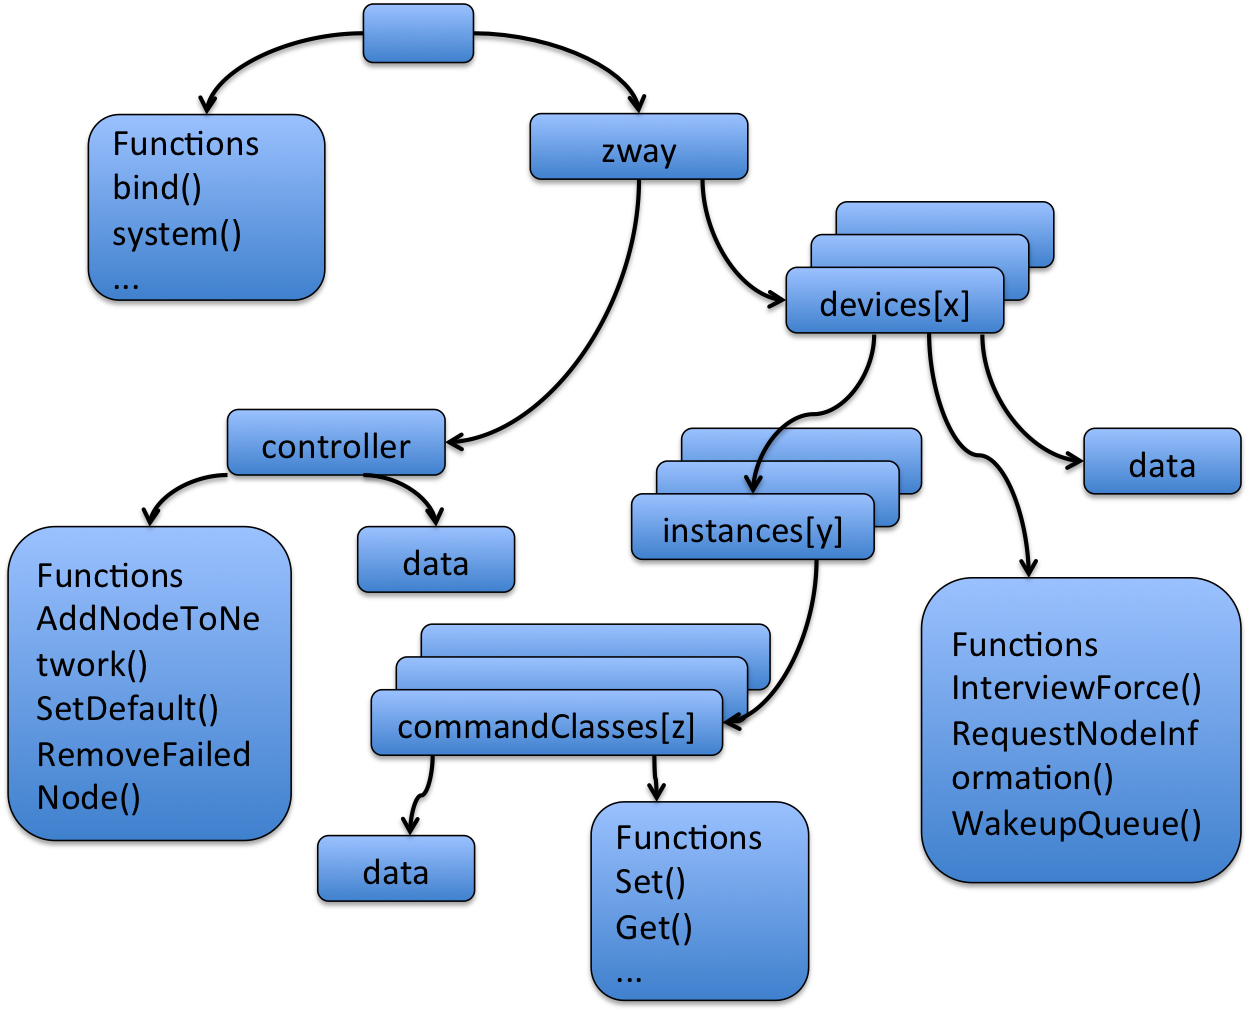
\includegraphics[width=0.9\textwidth]{pngs/cap11/zwayblocks.png}
\caption{\zway Object Tree Structure}
\label{zwaystructure}
\end{center}
\end{figure}

\subsubsection {The Data and Method Tree}

The root of the data tree has two important child objects:
\begin{itemize}
\item controller, this is the data object that holds all data and methods 
(commands, mainly function classes) related to the \zway controller as such 
\item devices array, this is the object array that holds the device -specific 
data and methods (commands, mainly command classes).
\end {itemize}


\subsection{Timing behavior of Z-Wave data}

\textbf{Please note that all status variables accessible on the Z-Wave Device APIs
are only proxy of the real value in the network.}

To transport data between the real wireless device and the GUI multiple 
communication instances are involved. The complexity of this communication 
chain will be explained in the following example:

\begin{figure}
\begin{center}
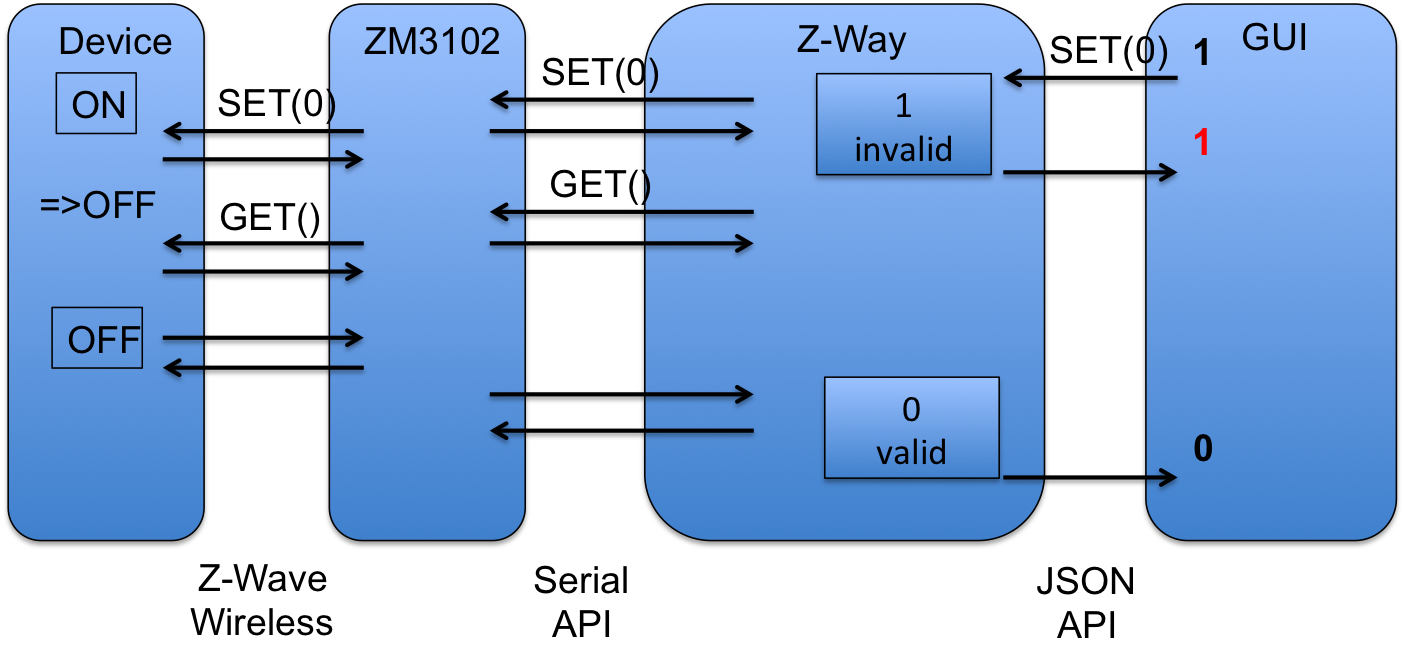
\includegraphics[width=0.9\textwidth]{pngs/cap11/zway2en.png}
\caption{\zway Timings}
\label{zwaytimings}
\end{center}
\end{figure}

Assuming the GUI shows the status of a remote switch and allows changing the switching 
state of this device. When the user hits the switching button, he expects to see the 
result of his action as a changing status of the device in the GUI. The first step is 
to hand over the command (SET) from the GUI to \zway using the JSON interface. \zway 
receives the command and will confirm the reception to the GUI. \zway recognizes that 
the execution of the switching command will likely result in a change of the status 
variable However \zway will not immediately change the status variable but invalidate 
the actual value (mark as outdated). This is the correct action because at the moment 
when the command was received the status on the remote device has not been changed yet 
but the status of the switch is now unknown.
If the GUI polls the value it will still see the old value but marked as invalid. \zway 
will now hand over the switching command to the Z-Wave transceiver chip. Since it is 
possible that there are other command waiting for execution (sending) by the Z-Wave 
transceiver chip the job queue is queuing them and will handle certain priorities if 
needed. \zway has recognized that the command will likely change the status of the remote 
device and is therefore adding another command to call the actual status after the 
switching command was issued.
The transceiver is confirming the reception of the command and this confirmation is noted 
in the job queue. This confirmation however only means that the transceiver (Z-Wave chip) 
has accepted the command and does neither indicate that the remote device has receives it 
nor even confirming that the remote device has executed accordingly.
The transceiver will now try to send the command wirelessly to the remote device. A 
successful confirmation of the reception from the remote device is the only valid indicator
 that the remote device has received the command (again, not that it was executed!).
The second command (GET) is now transmitted the very same way and confirmed by the 
remote device. This device will now sent a REPORT command back to \zway reporting the 
new status of the switching device. Now the transceiver has to confirm the reception. 
The transceiver will then send the new value to the \zway engine by issuing commands 
via the serial interface. \zway receives the report and will update the switching 
state and validate the value. From now on the GUI will receive a new state when polling.

\subsection{Executing Commands}
\label{jsapiexec}

JSON API allows executing commands on the server side using HTTP POST or GET requests. 
The command to execute is taken from the URL.

All functions are executed in form


\murl{http://YOURIP:8083/Run/ZWaveAPI*}.

The best way to learn about the commands and the data is to use the \zweui plus 
a JavaScript Debugger to see the command the AJAX code of the \zweui sends to the 
\zway server backend. Additionally the Z-Wave Expert User Interface provides nice and 
convenient vizualization of all commends (both command classes and function classes).

All access to the webserver require authentication of the user. Please refer to Chapter
\ref{cap:authentication} for details how to authenticate.

\subsubsection{Function Class Commands}


\begin{figure}
\begin{center}
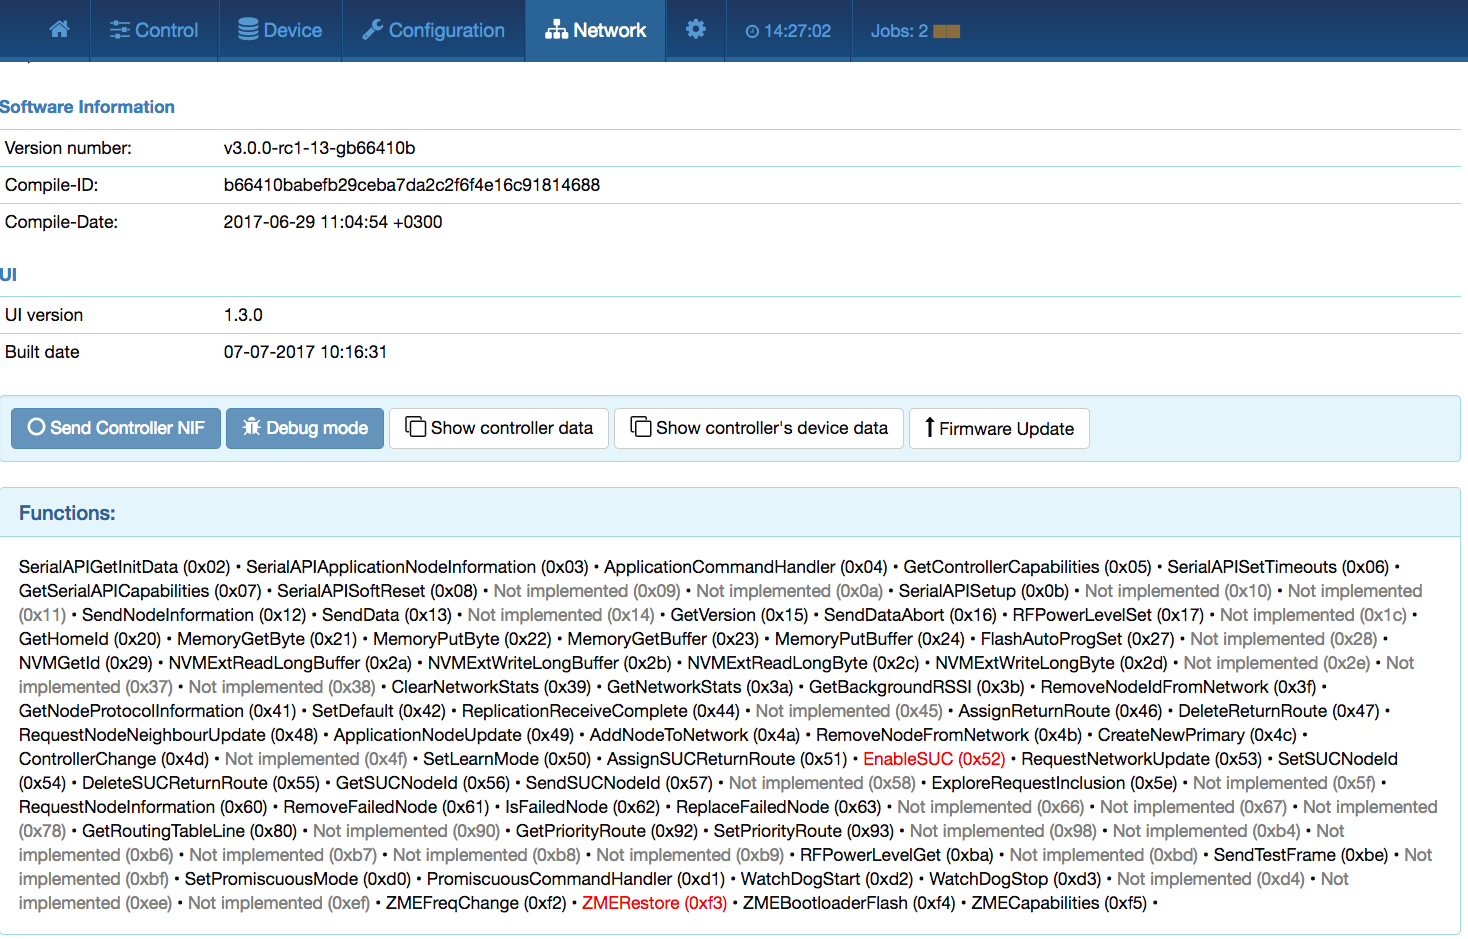
\includegraphics[width=0.9\textwidth]{pngs/cap11/dev3.png}
\caption{\zway Function Classes}
\label{dev3}
\end{center}
\end{figure}

Figure \ref{dev3} shows the Controller Info Page in Network menu with a list of all 
function classes implemented. The complete reference of the parameters and return 
values of the functions classes you find in annex \ref{FunctionClasses}.

Assuming there is a function class ``SerialAPIGetInitData’’ it is possible to call 
the function by calling the URL

\murl{/ZWaveAPI/Run/SerialAPIGetInitData(0)}

in the web browser. In case the function was completed successfully, a simple ``null’’ 
is returned; otherwise, an error code is provided.

\subsubsection{Device Command Class Commands}


\begin{figure}
\begin{center}
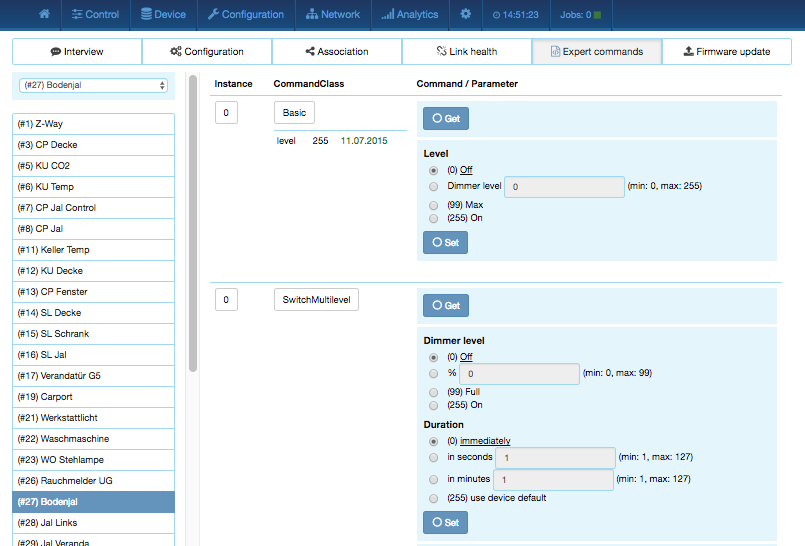
\includegraphics[width=0.9\textwidth]{pngs/cap7/eui35.png}
\caption{\zway Expert Command Class Commands}
\label{dev0}
\end{center}
\end{figure}

In the same manner, it is possible to send a command to a device using one of its command 
classes. The \zweui provides a general menu item called Expert Commands as 
shown in Figure \ref{dev0}. \zway reads out all command classes and its functions and
 provides here a complete list of command lass-specific commands. The debug window will 
 reveal the syntax if the complete command class reference in Annex \ref{ccs} is not 
available or too inconvenient to use.


For example, to switch ON a device no 2 using the command class BASIC, it is possible to write:

\begin{quote}
\small{\texttt{/ZWaveAPI/Run/devices[2].instances[0].commandClasses[0x20].Set(255)}}
\end{quote}
or

\begin{quote}
/ZWaveAPI/Run/devices[2].instances[0].Basic.Set(255)
\end{quote}

The \zweui has a JavaScript command 
\begin{quote}
\cmdline{runCmd($<$command$>$)}
\end{quote}
to simplify such operations. 
This function is accessible in the JavaScript console of your web browser 
(in Chrome you find the JavaScript console under View-$>$Debug-$>$JS Console). 
Using this feature, the command in JS console would look like

\begin{quote}
\cmdline{runCmd('devices[2].instances[0].Basic.Set(255)')}
\end{quote}


The usual way to access a command class is using the format \\'devices[nodeId].instances[instanceId].
commandClasses[commandclassId]'.
There are ways to simplify the syntax:

\begin{itemize}
\item ``devices[nodeId].instances[instanceId].Basic’’ is equivalent to \\
``devices[nodeId].instances[instanceId].commandClasses[0x20]’’
\item the instances[0] can be obmitted: 
``devices[nodeId].instances[instanceId].Basic’’ then turns into ``devices[nodeId].Basic’’
\end{itemize}


\subsubsection{Accessing Data}

The data model or data holder object as described is Section \ref{datamodel} can be 
accessed completely using the \zweui. The two 
buttons \keystroke{Show controller Data} and \keystroke{Show controllers device data} in 
\menu{Network > Controller
Info} of \zweui as shown in Figure \ref{dev3}  lists all variables of the 
controller as such. One structure is controller-specific and one other structure is the 
data of the controller as node of the Z-Wave network.
All nodes of the Z-Wave network have the very same data structure beside their individual 
array of instances and command classes per instance. This data model for the individual 
devices can be access using \keystroke{Configuration > Show Interview results} in \zweui. 
Figure \ref{dev1} shows this dialog. On the top of the window there is a button with 
the devices name. This button reveals the data structure of the individual device 
as shown in Figure \ref{dev2}.

\begin{figure}
\begin{center}
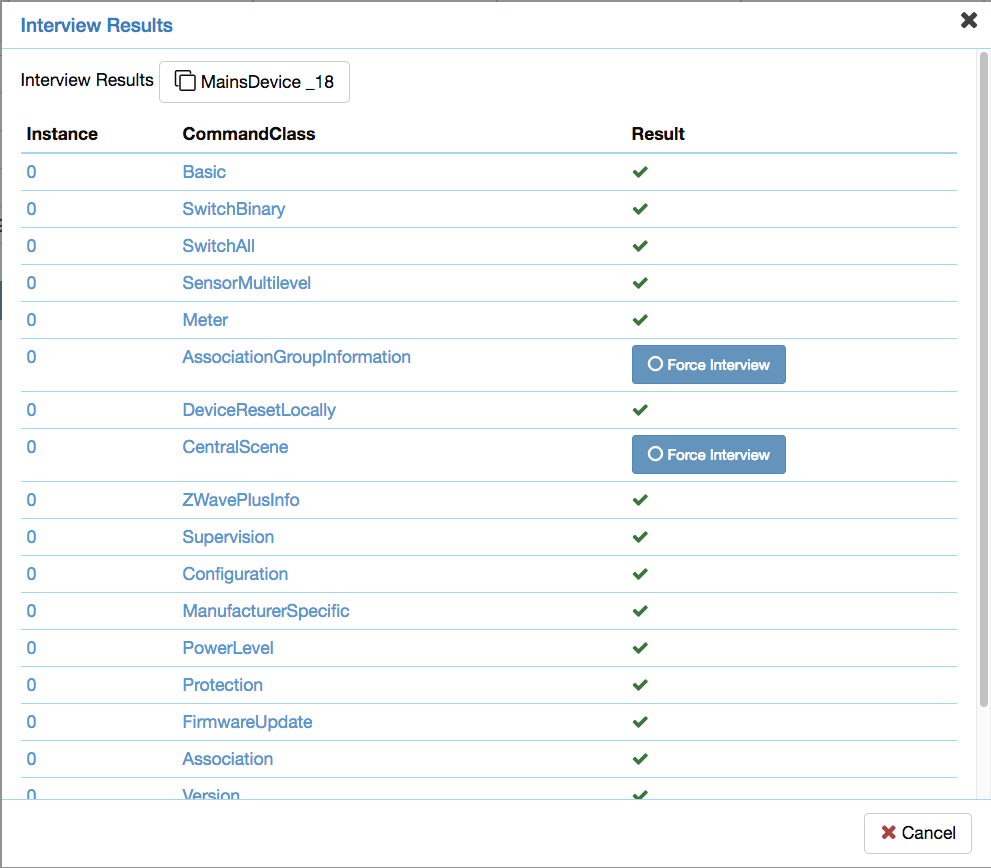
\includegraphics[width=0.9\textwidth]{pngs/cap11/dev1.png}
\caption{Command Class Inerview overview}
\label{dev1}
\end{center}
\end{figure}


\begin{figure}
\begin{center}
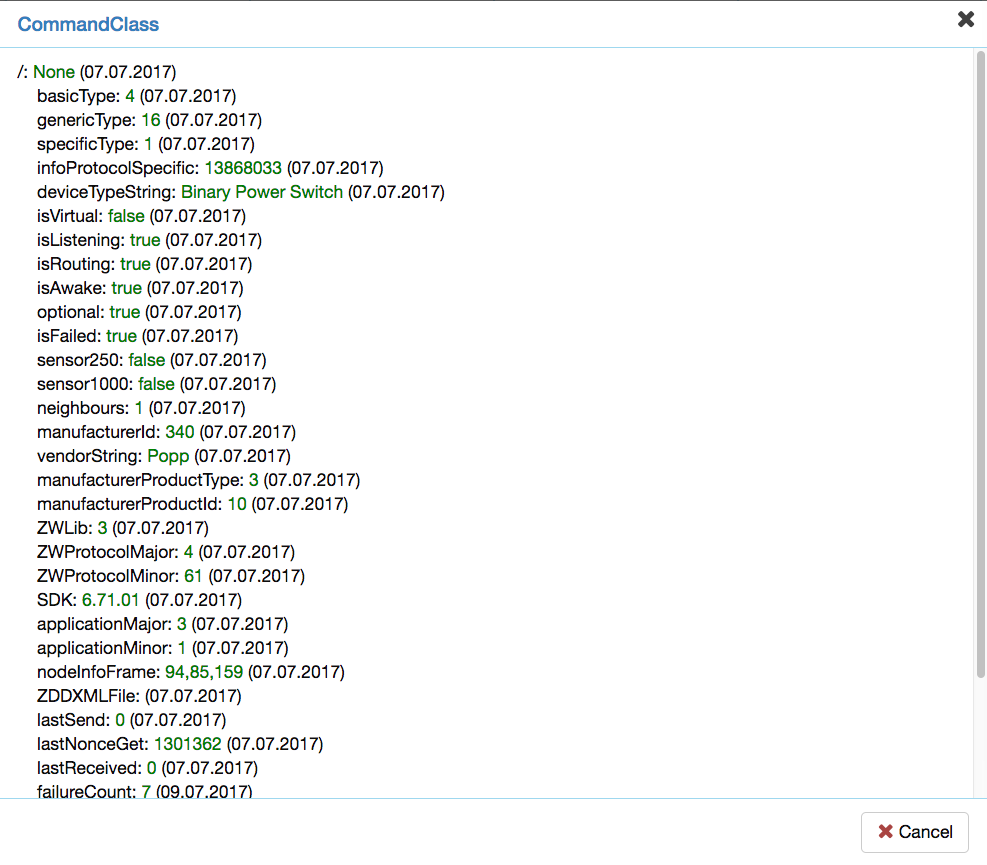
\includegraphics[width=0.9\textwidth]{pngs/cap11/dev2.png}
\caption{Command Class Variables in \zweui}
\label{dev2}
\end{center}
\end{figure}

The dialog has the list of all command classes and clicking on the name of the command 
class will open a sub dialog showing the data of the commend class. Each command class 
has some permanent values:

\begin {itemize}
\item supported: This indicates if this command classes is supported or controlled only
\item version: This is the version number of the command class as detected during the 
device interview using the command class ``VERSION’’
\item security: Indicates if this command class is within the security environment
\item interviewDone: This flag indicates if the interview of this particular command classes passed
\item interviewCounter: This is a helper variable that is counted down on every attempt to 
interview the devices. Its default value is 10. If it reaches 0 (10 unsuccessful attempts), 
\zway will give up interviewing. This makes sure that \zway is not blocked by devices 
with wrong implementation not passing interview.
\end{itemize}

Any data holder object has properties value, updateTime, invalidateTime, name, but for 
compatibility with JS and previous versions we have valueOf() method (allows 
omitting .value in JS code, hence write "data.level == 255"), updated (alias to updateTime), 
invalidated (alias to invalidateTime).


\subsubsection{/ZWaveAPI/Data/$<$timestamp$>$}

Returns an associative array of changes in \zway data tree since $<$timestamp$>$. The array 
consists of ($<$path$>$: $<$JSON object$>$) object pairs. The client is supposed to assign 
the new $<$JSON object$>$ to the subtree with the $<$path$>$ discarding previous content 
of that subtree. Zero (0) can be used instead of $<$timestamp$>$ to obtain the full \zway 
data tree.

The tree have same structure as the backend tree (Figure \ref{zwaystructure}) with one 
additional root element "updateTime" which contains the time of latest update. This 
"updateTime" value should be used in the next request for changes. All timestamps 
(including updateTime) corresponds to server local time.

The object looks like:
\begin{listingverbatim}[JSON Data Structure]
\{
  "[path from the root]": [updated subtree],
  "[path from the root]": [updated subtree],
  ...
  updateTime: [current timestamp]
}
\end{listingverbatim}

Examples for Commands to update the data tree look like:

\begin{quote}Get all data: /ZWaveAPI/Data/0\end{quote}

\begin{quote} Get updates since 134500000 (Unix timestamp): /ZWaveAPI/Data/134500000\end{quote}

Please note that during data updates some values are updated by big subtrees. For 
example, in Meter Command Class value of a scale is always updated as a scale 
subtree by [scale].val object (containing scale and type descriptions).


\subsubsection{/ZWaveAPI/InspectQueue}

This function is used to visualize the \zway job queue. This is for debugging only but 
very useful to understand the current state of \zway engine.

The information given on this page is only relevant for advanced Z-Wave developers and 
for debugging.

The table shows the active jobs with their respective status and additional information.

\begin{table}
\begin{tabular}{|p{0.3\textwidth}|p{0.6\textwidth}|}
\hline
n	&This column shows the number of sending attempts for a specific job. \zway tries three times to dispatch a job to the transceiver.\\
\hline
W,S,D: & This shows the status of the job. If no indicator is shown the job is in active state. This means that the controller just tries to execute the job. ``W’’ states indicated that the controller believes that the target device of this job is in deep sleep state. Jobs in ``W’’ state will remain in the queue to the moment when the target device announces its wakeup state by sending a wakeup notification to the controller. Jobs in ``S’’ state remain in the waiting queue to the moment the security token for this secured information exchanged was validated.
``D’’ marks a job as done. The job will remain in the queue for information purposes until a job garbage collection removed it from the queue.\\
\hline
ACK:& shows if the Z-Wave transceiver has issued an ACK message to confirm that the message was successfully received by the transceiver. This ACK however does not confirm that the message was delivered successfully. A successful delivery of a message will result in a “D” state of this particular job.
If the ACK field is blank, then no ACK is expected. A “.” indicates that the controller expects an ACK but the ACK was not received yet. A “+” indicates that an ACK was expected and was received.\\
\hline
RESP	&shows if a certain command was confirmed with a valid response. Commands are either answered by a response or a callback.
If the RESP field is blank, then no response is expected. A ``.’’ indicates that the controller expects a response, but the response has not been received yet. A ``+’’ indicates that a response was expected and has been received.\\
\hline
Cbk	&If the Cbk field is blank, then no callback is expected. A “.” indicates that the controller expects a Callback but the Callback was not received yet. A “+” indicates that a Callback was expected and was received.\\
\hline
Timeout	&Shows the time left until the job is de queued \\
\hline
Node Id	&shows the ID of the target node. Communication concerning the network, like inclusion of new nodes, will have the controller nodeID as a target node ID. For command classes command the node ID of the destination Node is shown. For commands directed to control the network layer of the protocol, the nodeID is zero. \\
\hline
Description	&shows a verbal description of the job \\
\hline
Progress	&shows a success or error message depending on the delivery status of the message. 
Since \zway tries three times to deliver a job up to 3 failure messages may appear.
Buffer: It shows the hex values of the command sent within this job \\

\hline
\end{tabular}
\caption{Parameters of the Job Queue Vizualization}
\label{c1:queuecommands}
\end{table}

Table \ref{c1:queuecommands} summarizes the different values displayed on the Job Queue 
visualization. While this info is certainly not relevant for end users of the system it 
is a great debug tool.

\subsubsection{Handling of updates coming from \zway}

A good design of a user interface is linking UI objects (label, textbox, slider, ...) to a certain 
path in the tree object. Any update of a subtree linked to user interface will then update the user interface
too. This is called bindings.

For web applications \zway contains a library called jQuery.triggerPath (extention of 
jQuery written by Z-Wave.Me), that allows making such links between objects in the 
tree and HTML DOM objects. Use

\begin{quote}var tree;\end{quote}
\begin{quote}jQuery.triggerPath.init(tree);\end{quote}

during web application initialization to attach the library to a tree object. Then run

\begin{quote}jQuery([objects selector]).bindPath([path with regexp], [updater function],
[additional arguments]);\end{quote}

to make binding between path changes and updater function. The updater function would be 
called upon changes in the desired object with this pointing to the DOM object itself, 
first argument pointing to the updated object in the tree, second argument is the exact 
path of this object (fulfilling the regexp) and all other arguments copies additional 
arguments. RegExp allows only few control characters: * is a wildcard, (1|2|3) - is 1 or 2 or 3.

\textbf{Please note that the use of the triggerpath extension is one option to handle 
the incoming data. You can also extract all the interesting values right when the 
data is received and bind update functions to them.}

\subsubsection{Handling S2 inclusion process}

Security S2 inclusion process require additional interaction with the user
during inclusion process. In addition to putting the device in Learn Mode
and \zway in Add mode the user will be asked to grant different Security S2 keys
and enter the PIN code.

To implement Security S2 inclusion process in your own app follow the steps
below:
\begin {itemize}
\item Include the device
\item Check if it supports S2 (if the Command Class exists)
\item If Smart Start is in progress, nothing to be done --- \zway will handle
everything automatically
\item Wait for {\small{\texttt{devices[N].instances[0].commandClasses[159].data.requestedKeys}}} to become True
\item Check {\small{\texttt{data.requestedKeys}}} children and set {\small{\texttt{data.grantedKeys}}} children accordingly. In most cases you would just copy from requested to granted
(grant all keys the device requested for).
\item Set {\small{\texttt{data.grantedKeys}}} to True to notify \zway that you are done with keys selection
\item Wait for {\small{\texttt{data.publicKeyAuthenticationRequired}}} to be set. If False (device was not granted Access or Authenticated keys), copy in
{\small{\texttt{data.publicKeyVerified}}} the {\small{\texttt{data.publicKey}}} (it is recommended to show first two bytes in decimal form to the user to confirm). Otherwise copy and fill first two bytes with the PIN code.
\item A failed Security S2 interview will result in {\small{\texttt{data.securityAbandoned}}} to be
set to True. A successfull one will have {\small{\texttt{data.securityAbandoned}}}
equal to False and {\small{\texttt{data.interviewDone}}} equal to True.
\end{itemize}


\section{C-Library API and a general view on the \zway file structure}
\label{clevelapi}

\subsection{Files in the /zway folder}
\label{c11:zwayfolder}
\index{Folder}
\index{Folder Structure}
\index{Files}
\index{File Descriptions}

\zway keeps all files in one folder with exception of the log files. In Unix based 
platforms such as Linux PC, Raspberry Pi or open WRT the standard install folder 
is usually \cmdline{/opt/zway-server}. The logfile is typically placed in 
\cmdline{/var/log/z-way-server.log} but this location of the log file can be 
reconfigured in the config file.

On Windows, the installation wizard asked where to place \zway and where to place the log file.

Right after installation, the standard folder has the following content:

{\footnotesize
\begin{forest}
  for tree={
    font=\ttfamily,
    grow'=0,
    child anchor=west,
    parent anchor=south,
    anchor=west,
    calign=first,
    edge path={
      \noexpand\path [draw, \forestoption{edge}]
      (!u.south west) +(7.5pt,0) |- node[fill,inner sep=1.25pt] {} (.child anchor)\forestoption{edge label};
    },
    before typesetting nodes={
      if n=1
        {insert before={[,phantom]}}
        {}
    },
    fit=band,
    before computing xy={l=15pt},
  }
[z-way-server
[automation: The JavaScript sub system]
[config: Various configuration xml files]
[htdocs: The web servers doc directory]
[libs: The binary libs such as libzway etc.]
[libzway Header files for libzway and other libs]
[modules: binary modules]
[modules-includes: header file for binary modules]
[translations: XMLs mapping Ids to text]
[ZDDX: Device Description Files]
[z-get-tty-config: Config for utility]
[ChangeLog]
[config.xml: Main config file]
[z-get-tty: Utility]
[z-way-server: Main Application]
]
\end{forest}
}

\subsubsection{config.xml - the main config file}

The main config file in the root folder has XML file format. If only allows setting the 
log level (0 = log all, 9 = log almost nothing), the path to the log file and a debug 
port if needed. Don't change the setting for automation folder unless you really 
know what you do and why.

This is an example for the standard config.xml displaying all log right into the console.
\begin{listingverbatim}[config.xml]
<config>
    <automation-dir>automation</automation-dir>
    <log-file></log-file>
    <log-level>0</log-level>
    <debug-port>0</debug-port>
</config>
\end{listingverbatim}

\subsubsection{config: Various configuration xml files}

This subfolder has the following structure:

{\footnotesize
\begin{forest}
  for tree={
    font=\ttfamily,
    grow'=0,
    child anchor=west,
    parent anchor=south,
    anchor=west,
    calign=first,
    edge path={
      \noexpand\path [draw, \forestoption{edge}]
      (!u.south west) +(7.5pt,0) |- node[fill,inner sep=1.25pt] {} (.child anchor)\forestoption{edge label};
    },
    before typesetting nodes={
      if n=1
        {insert before={[,phantom]}}
        {}
    },
    fit=band,
    before computing xy={l=15pt},
  }
[config
[maps: legacy folder]
[zddx
		[HOMEID-DeviceData.xml: main storage for Z-Wave structure]
]
[Defaults.xml: Default Settings]
[Profiles.xml]
[Rules.xml]
]
\end{forest}
}
\\
The file \cmdline{Defaults.xml} allows defining various behavior of \zway, among them the appearance of \zway as secondary controller:

\begin{itemize}
\item AutoConfig: Flag if \zway shall interview the device right after inclusion (default = 1)
\item DeepInterview: Flag that Interview is only completed after all values are received 
back. This includes asking the device for all initial values of sensor or status data (default = 1)
\item SaveDataAfterInterviewSteps: Flag whether or not all device data will be saved after each interview step (default = 1)
\item TryToBecomeSIS: Will \zway try to become networks SIS if transceiver hardware allows it to (default = 1)?

\item SecureInterviewAsInclusionController: \zway will initiate interview as Inclusion Controller, if 0 - only as Primary/SIS
\item SecureInterviewAcceptedWithoutSchemeInherit: If 1 - \zway will not fail secure interview 
as secondary/inclusion controller if Scheme Inherit is not received, if 0 - fail interview as by Z-Wave protocol
\item SecureAllCCs: Always use Security if possible (even for CCs allowed as non-secure)
\item DeviceReplyTimeout: Delay to wait (in seconds) for a device to reply with a REPORT on a GET command
\item DeviceRelaxDelay: Delay between two subsequent packets sent to one device, measured 
in ticks (~10 ms). Some slow devices might need about 10 to respond correctly to burst of packets
\item SerialAPITimeout: Extra time to be added to Serial API timouts. Set up to 1.0-3.0 
sec in case of slow channel toward Z-Wave chip (e.g. in cloud applications) 
\item Command Class-Specific Settings
\begin{itemize}
\item Wakeup -> WakeupInterval: Default Wakeup Interval
\item Scene Actuator Conf -> Max Scenes: Maximum number of Scenes supported
\item Scene Controller Conf -> Max Scenes: Maximum number of Scenes supported
\item Protection -> Mode: Default Protection Mode
\item SensorMultilevel -> Fahrenheit: Flag what temperature scale is used
\item SwitchAll -> Mode: Default Switch All mode
\item MultiCmd -> MaxNum: The maximum number of commands within multi-command encapsulation. 
The optimal value would be even, but there are many broken devices in the market that do 
not support this. A lower number means less efficient but more robust against faulty devices.
\item Firmware Update -> Fragment Size: Fragment size on 3rd gen RaZberry and 3rd gen UZB 
cannot be more than 32 (max packet size was 37, with possible CRC it gives 32). On UZB 
and new 5gen it can be up to 40 bytes
\item ThermostatSetPoint: -> Fahrenheit: Flag what temperature scale is used
\end{itemize}

\item Controller: Description of how \zway will behave as a device in the network. This entry has the following subentries:

\begin{itemize}
\item NodeInformationFrame: The command class \zway is described as ``supported’’ in the network
\item SecureNodeInformationFrame: Command Classes available in secure environment
\item InstanceNodeInformationFrame: Command Classes in Instances if Multi Channel is emulated
\item VersionID =iD: Versions to be reported in Command Class Version Get Command for all Command Classes announced in NIF
\item Name: Default Node Name reported by NodeNaming Report
\item Location Default Node Location of Controller reported by NodeNaming Report
\item AppVersion: Application Version reported by ManufacturerSpecific Report
\item Manufacturer\ Specific: Values report by ManufacturerSpecific Report
\item SpecificDeviceClass: Specific Device Class reported
\item GenericDeviceClass: Generic Device Class reported
\item Icons: Z-Wave Plus Icons
\item Lifeline: Defines how many devices will be in Lifeline Association Group
\item CommandClassSupportedVersion: Defines the version numbers of the supported command classes
\item Channels: Defines the simulated channels
\end{itemize}

\end{itemize}

The file \cmdline{Profiles.xml} contains the EnOcean profile definition. This clearly 
reflects the official profile definitions published by the EnOcean alliance.

The file \cmdline{Rules.xml} is a legacy file.

\subsubsection{translations: XMLs mapping Ids to text}

{\footnotesize
\begin{forest}
  for tree={
    font=\ttfamily,
    grow'=0,
    child anchor=west,
    parent anchor=south,
    anchor=west,
    calign=first,
    edge path={
      \noexpand\path [draw, \forestoption{edge}]
      (!u.south west) +(7.5pt,0) |- node[fill,inner sep=1.25pt] {} (.child anchor)\forestoption{edge label};
    },
    before typesetting nodes={
      if n=1
        {insert before={[,phantom]}}
        {}
    },
    fit=band,
    before computing xy={l=15pt},
  }
[translations
[AEC.xml: Advanced Energy Framework]
[Alarms.xml: Alarm conditions]
[BarrierSignals.xml]
[ColorCapabilities.xml]
[DeviceClasses.xml: Z-Wave Classic Device Classes]
[LocEvents.xml: Door Lock Events]
[Scales.xml: Sensor Multilevel and Meter Scales]
[SDKIds.xml: Major Minor into SDK versions]
[ThermostatModes.xml]
[VendorIds.xml: Vendor Id into Vendor Name]
[ZWavePlus.xml: Z-Wave Plus Role Types and Network Types]
]
\end{forest}
}

All files in this subfolder are XML files and some of them require local language 
translations, as described in Chapter \ref{sec:translation}.

\subsubsection{ZDDX: Device Description Files}

ZDDX files (Z-Wave Device Description XML Files) are XML files containing verbal 
description of a specific Z-Wave device that cannot be called from the device itself 
during the interview process: They are:

\begin{itemize}

\item The naming of Association Groups. Modern Z-Wave device provides them in English 
language using the Association Group Information Command Class. The ZDDX file provides this 
information for older devices and in various languages.

\item Configuration Parameters and Values: It is always possible to set a configuration 
value knowing the integer values from the device manual. \zway offers a convenient way 
to set Z-Wave configuration values utilizing the information from ZDDX files.

\item An Image of the device.

\item Information on inclusion, exclusion and wakeup processes.

\end{itemize}

It is possible to add your own ZDDX files, but \zway uses an index file ZDDX.indx to access them. Once a new file is added, run \cmdline{python MakeIndex.py}.

Chapter \ref{newddr} explain how to add and to submit new own ZDDX files and how to extend them.

\subsubsection{Htdocs: The web servers document folder}

{\footnotesize
\begin{forest}
  for tree={
    font=\ttfamily,
    grow'=0,
    child anchor=west,
    parent anchor=south,
    anchor=west,
    calign=first,
    edge path={
      \noexpand\path [draw, \forestoption{edge}]
      (!u.south west) +(7.5pt,0) |- node[fill,inner sep=1.25pt] {} (.child anchor)\forestoption{edge label};
    },
    before typesetting nodes={
      if n=1
        {insert before={[,phantom]}}
        {}
    },
    fit=band,
    before computing xy={l=15pt},
  }
[htdocs : web server doc folder
	[config: link from /config into web space]
	[ZDDX: link from /ZDDX into web space]
	[expert: Z-Wave Expert User Interface]
	[smarthome: Smart Home User Interface]
	[translation]
	[index.html]
]
\end{forest}
}

This subfolder is the root folder of the embedded webserver. The index.html redirects to smarthome/index.html.

\subsubsection{automation: The JavaScript sub system}

{\footnotesize
\begin{forest}
  for tree={
    font=\ttfamily,
    grow'=0,
    child anchor=west,
    parent anchor=south,
    anchor=west,
    calign=first,
    edge path={
      \noexpand\path [draw, \forestoption{edge}]
      (!u.south west) +(7.5pt,0) |- node[fill,inner sep=1.25pt] {} (.child anchor)\forestoption{edge label};
    },
    before typesetting nodes={
      if n=1
        {insert before={[,phantom]}}
        {}
    },
    fit=band,
    before computing xy={l=15pt},
  }
[automation
[classes: Some base classes of the JS system]
[core: The core classes of the JS system]
[defaultConfigs: A collection of default config.json files]
[lang: Translations of JS system messages]
[lib: Some utility scripts of the JS system]
[modules: The preinstalled apps]
[userModules: Downloaded apps
	[uploadModule.sh: Utility to upload own created apps]
]
[storage: The central folder to store all user data and settings
	[configjson-XXXXXXX: Configuration Settings of Smart Home UI]
	[dedevicesjson-XXXXXXX: complete device description in German)]
	[endevicesjson-XXXXXXX: complete device description in English]
	[expertconfigjson-XXXXXXX: Configuration Settings of Expert UI]	
	[history-XXXXXXX: Data for 24 hour history display]
	[...: more json files containing data]		
]
]
\end{forest}
}

The subfolder for automation contains the whole JavaScript (JS) subsystem including the
\begin{itemize}
\item source code of the software core (classes, core, lib),
\item the storage for the apps (modules, user modules),
\item the central storage for configs, images, uploads, history, logging, etc.,
\item some default files for factory default reset and recovery from failures.
\end{itemize}

The most sensitive file is configjson-XXX since it contains the information about the user 
accounts including login name, password, and recovery email.

For more information about the creation of new modules that will be placed into the user 
modules, please refer to Chapter \ref{developownapps}.

\subsection{The use of  the C-Library}


The \zway library is a middleware between Silicon Labs \zwave transceiver and your application. 
\zway offers pretty high level API to control \zwave devices and manage wireless network.

Interaction with the library covers three aspects:
\begin{itemize}
\item sending commands to \zwave devices;
\item sending network management commands to the transceiver;
\item receiving updates from the network.
\end{itemize}

\subsubsection{Sending commands}

Every command request generates an outgoing packet (job). Before generating a packet, 
library will validate parameters and check whether the command is supported by the recipient. 
In case of failure command will return error immediately.

Once a job is generated, it is placed into outgoing queue for future send. The queued jobs 
are handled internally by \zway engine according to commands priorities, nodes states 
and capabilities, transceiver state etc.

Once the job is sent, it must be first confirmed it was successfully delivered to 
the \zwave stack, and then confirmed it was delivered to the recipient. All these operations are 
performed asynchronously, so command may provide a callback function to call in case of 
success or failure if it is needed to know delivery result.

After the delivery was confirmed, command is considered executed. If it was a state 
request command (i.e. \texttt{SensorMultilevel Get}), response packet may be delayed 
(or even not sent at all), so command's success/failure callbacks cannot be used to get 
requested state immediately.

\subsubsection{Receiving updates}

All incoming packets from the \zwave network are automatically parsed by \zway and stored in 
special variables called data holders. Data holder is a named variable that stores a value 
along with its data type and time the value was last updated and "invalidated". Each data
holder may also contain a set of child data holders, so they form a hierarchical data 
storage. Data holders also support callbacks, so custom code may be executed each time 
the value is updated.


For example, \texttt{level} data holder stores dimming level of a dimmer. Once application 
executes a \texttt{Get} command for that dimmer, \zway will update \texttt{invalidateTime} property on 
the \texttt{level} data holder, so application knows the current value is assumed to be 
outdated, but the new one was not received yet.

Once \zway received a packet with new value of the dimmer, it will store it in \texttt{level 
data holder} and update \texttt{updateTime} property. Since \texttt{updateTime} is 
greater that \texttt{invalidateTime}, the value is considered valid now.

\zwave device can also send unsolicited state reports to controller (without a request 
from controller's side; e.g. due to local operation or periodically). Due to asynchronous 
nature of \zwave protocol, controller can't tell whether the packet was sent unsolicited 
or it is a response to the previous command. So unsolicited packet will be handled the 
same way exactly.

\subsubsection{Command Classes}

\zway inherits structure of \zwave protocol and divides data holders and commanda on
different Command Classes (CC). Command Classes are building blocks of \zwave functionality.
For example, dimming is provided by Command Class \texttt{SwitchMultilevel}, relay 
operation by Command Class \texttt{SwitchBinary}, sensors by command class 
\texttt{SensorMultilevel} and \texttt{SensorBinary} etc. Please consult \zwave 
protocol basics to understand \zwave Command Classes.

All Command Classes share a minimal subset of common data holders:

\begin{itemize}
\item \texttt{supported} says if CC is supported by the device (it implements that 
functionality) or only controlled (it can control other devices implementing that 
functionality).
\item \texttt{version} stores version of the CC. Used internally to know how to deal 
with that Command Class.
\item \texttt{security} tells if CC communications should be encrypted using \zwave 
AES security mechanism.
\item \texttt{interviewDone} and \texttt{interviewCounter} describe the status of 
initial interview process during which \zway asks the device about its CC capabilities. 
If the interview is incomplete, \zway might fail to use some Command Classes with this 
device. All \zwave certified devices MUST pass interview process.
\end{itemize}

All the other data holders are specific to each Command Class. For example, 
\texttt{SwitchMultilevel Command Class} contains \texttt{level} data holder, 
\texttt{SensorBinary} has two-level storage, grouping data by sensor types:
\texttt{ 0 -> {sensorTypeString, level}, 5 -> {sensorTypeString, level}, ... }
where type identifiers are \zwave specific constants. Every \zwave specific constant 
value will have corresponding verbal description (in case of \texttt{SensorBinary} it is in 
\texttt{sensorTypeString} data holder).

Some Command Classes are hidden under the hood of \zway: 
\texttt{MultiCmd, Security, CRC16, MultiChannel, ApplicationStatus}. They're handled 
internally by \zway software, and shouldn't be used directly.

Some Command Classes have no public APIs, but their data holders may be very useful 
in your application: \texttt{Association\-Group\-Information, Device\-Reset\-Locally,
Manufacturer\-Specific, Version, ZWavePlusInfo}.

All the remaing Command Classes have their \texttt{Get} and \texttt{Set }commands 
specific to functionality of the Command Class. Consult 
\texttt{CommandClassesPublic.h} header file for more info about available commands 
for different Command Classes and their meaning.

\subsubsection{Network management}

\zway offers API for network management operations: include new devices, exclude devices, 
discover neighbor devices, remove failed nodes, frequency selection, controller reset etc. 
These functions are described in \texttt{ZWayLib.h} header file.

\zway also provides a low level access to \zwave transceiver functionality through Silicon 
Labs Serial API. These functions are provided by Function Classes. You should use 
them only if you have deep knowledge of \zwave networking. Check 
\texttt{FunctionClassesPublic.h} for more info.

\subsubsection{Using \zway Library in C-Code}

To use \zway one need to include few header files:
\begin{listingverbatim}
\string#include <ZWayLib.h>
\string#include <ZLogging.h>
\end{listingverbatim}

\zway will need to know where to write the log to, so first of all you need to create 
logging context using \texttt{zlog\_create()} call. You can disable logging by passing NULL 
instead of logging context to \zway.

Then create new a \zway context using \texttt{zway\_init()}. It will only allocate memory, 
open log files, initialize internal structures. At this point you can already attach your 
handlers on new \texttt{device/instance/Command Class} creation (you will also be able 
to do it at any time later). Do it using \texttt{zway\_device\_add\_callback()} call. 

Warning: you should initialize ZWay pointer with NULL before passing it to \texttt{zway\_init}!

Executing \texttt{zway\_start()} will open serial port and start a new thread that 
will handle all communications with the transceiver. From now \zway can receive packets 
from the network, but can not parse them yet, since devices were not discovered yet. 
All received packets will just be queued to be parsed later after discovery process.

Last step to run \zway is \texttt{zway\_discover()} call. It will start communications 
with the \zwave transceiver and ask about devices in the network, their capabilities, 
network state etc. During discovery phase \zway will create structures for all devices and 
load saved data from file stored in \texttt{config/zddx} folder.

From now on, \zway is ready to operate. Incoming events will trigger callback functions 
attached by application, and executing commands will put new packets in the queue.

You will also need few other functions \texttt{zway\_is\_running(), zway\_is\_idle(), 
zway\_stop(), zway\_terminate()} to handler termination process.

\subsubsection{Handling secure inclusion}

Security S0 inclusion is completely handled by the Z-Way library.

Security S2 inclusion with Z-Way library requires user interaction. Z-Way offers various options:

\begin{itemize}
\item Use Smart Start technology:
   Call zway\_fc\_smart\_start\_enable() on start (this is done by the library on start).

   Add the device DSK using zway\_node\_provisioning\_dsk\_add() with a pointer to 16 bytes DSK and filled the NodeProvisioningData structure (instead of filling it one can fill it with zeros).

   The inclusion and key exchange will happen automatically on the device's power-up.

   All keys will be granted to the device.

   zway\_dsk\_string\_to\_bytes() can be used to convert AAAAA-BBBBB-...-HHHHH into 16 bytes.
\item Use the standard key grant process:

   After inclusion start subscribe to Command Classes creation (using zway\_device\_add\_callback() with CommandAdded flag) and wait for SecurityS2 creation. Then subscribe to the change of requestedKeys and puclickKey data holders on SecurityS2 Command Class data (using zdata\_add\_callback()).

   On requestedKeys change inspect inner data holders for the list of requested keys and fill all grantedKeys inner data holders (by setting TRUE or FALSE).

   Once done, set TRUE on the grantedKeys data holder.

   On puclickKey update check it against the DSK on the device (it is good to show the full key to the customer to allow full check).

   Copy the key in the puclickKeyVerified data holder to confirm. If publicKeyVerificationRequires is set to TRUE, the user should also be asked for the PIN code. This two-bytes code should replace the two leading zero bytes of the puclickKey.
\item Set the PIN and the list of desired security keys before inclusion:

    Just before starting the inclusion process with zway\_controller\_add\_node\_to\_network set data holders on the controller S2AutoInclude.pin=XXXXX (PIN number) and S2AutoInclude.keys=Y (-1 for all keys, 0x80 for S0 only, 0x01 for S2 Unauthenticated, 0x02 for S2 Authenticated, 0x04 for S2 Access, or any ORed combination to provide multiple keys)

    If there is no need for S2 Authentication or S2 Access keys, just specify pin=0 and keys=0x01. This will give S2Unauthenticated without entering the PIN code. keys=0x81 will grant S0 and S2 Unauthenticated.
\end{itemize}

\subsubsection{Sample project}

The link
\murl{https://storage.z-wave.me/z-way-server/z-way-test.tgz}

downloads a very simple test project using the \zway core library \texttt{libzway.so}. 
The project contains a simple \texttt{mains.c} plus a \texttt{Makefile}. A \zway installation is required 
too. To compile the test project, some requirements need to be met:
\begin {itemize}
\item GNU-based tool chain with a compiler, linker, etc.
\item Copy main.c and Makefile into the root folder of \zway
\item Check the path to library and header files and adapt the Makefile is needed
\item Make sure the following libraries are installed:
\begin {itemize}
\item libxml2 (apt-get install libxml2-dev)
\item libarchive (apt-get install libarchive-dev)
\item libcrypto (apt-get install libssl-dev)
\end {itemize}
\end {itemize}

Executing the Makefile will generate a binary executable \cmdline{z-way-test} in the same 
folder. If \zway was just downloaded the code will assume a virtual serial Z-Wave device 
on \cmdline{/dev/ttyUSB0}. if your virtual device is a different node, just make a 
symlink like \cmdline{ln -s /dev/ttyACM0 /dev/ttyUSB0} or change \texttt{main.c} file.

Now start the code from the folder with \cmdline{LD\_LIBRARY\_PATH=./libs ./z-way-test}. 
The header file \texttt{Z-Waylib.h} in \texttt{libzway} gives a brief explanation of the calls 
into the library. The demo file \texttt{main.c} demonstrates the use of the calls. 
Figure \ref{libterminal} shows the small help page of the test software.

\begin{figure}
\begin{center}
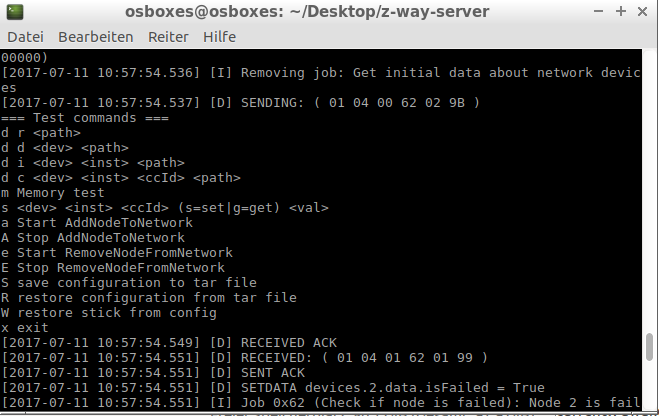
\includegraphics[width=0.9\textwidth]{pngs/cap11/libterminal.png}
\caption{Terminal running z-way-test}
\label{libterminal}
\end{center}
\end{figure}
